%!TEX root = ../../main.tex
\chapter{Box Model}
\label{cha:box_model}

This design manual utilizes the standard box model that consists of content, padding, border and margins as seen on Figure \ref{fig:box_model}. The main difference to notice is that \emph{margin} is the outer spacing and that \emph{padding} is the innser spacing on elements. 

\begin{figure}[h]
	\centering
	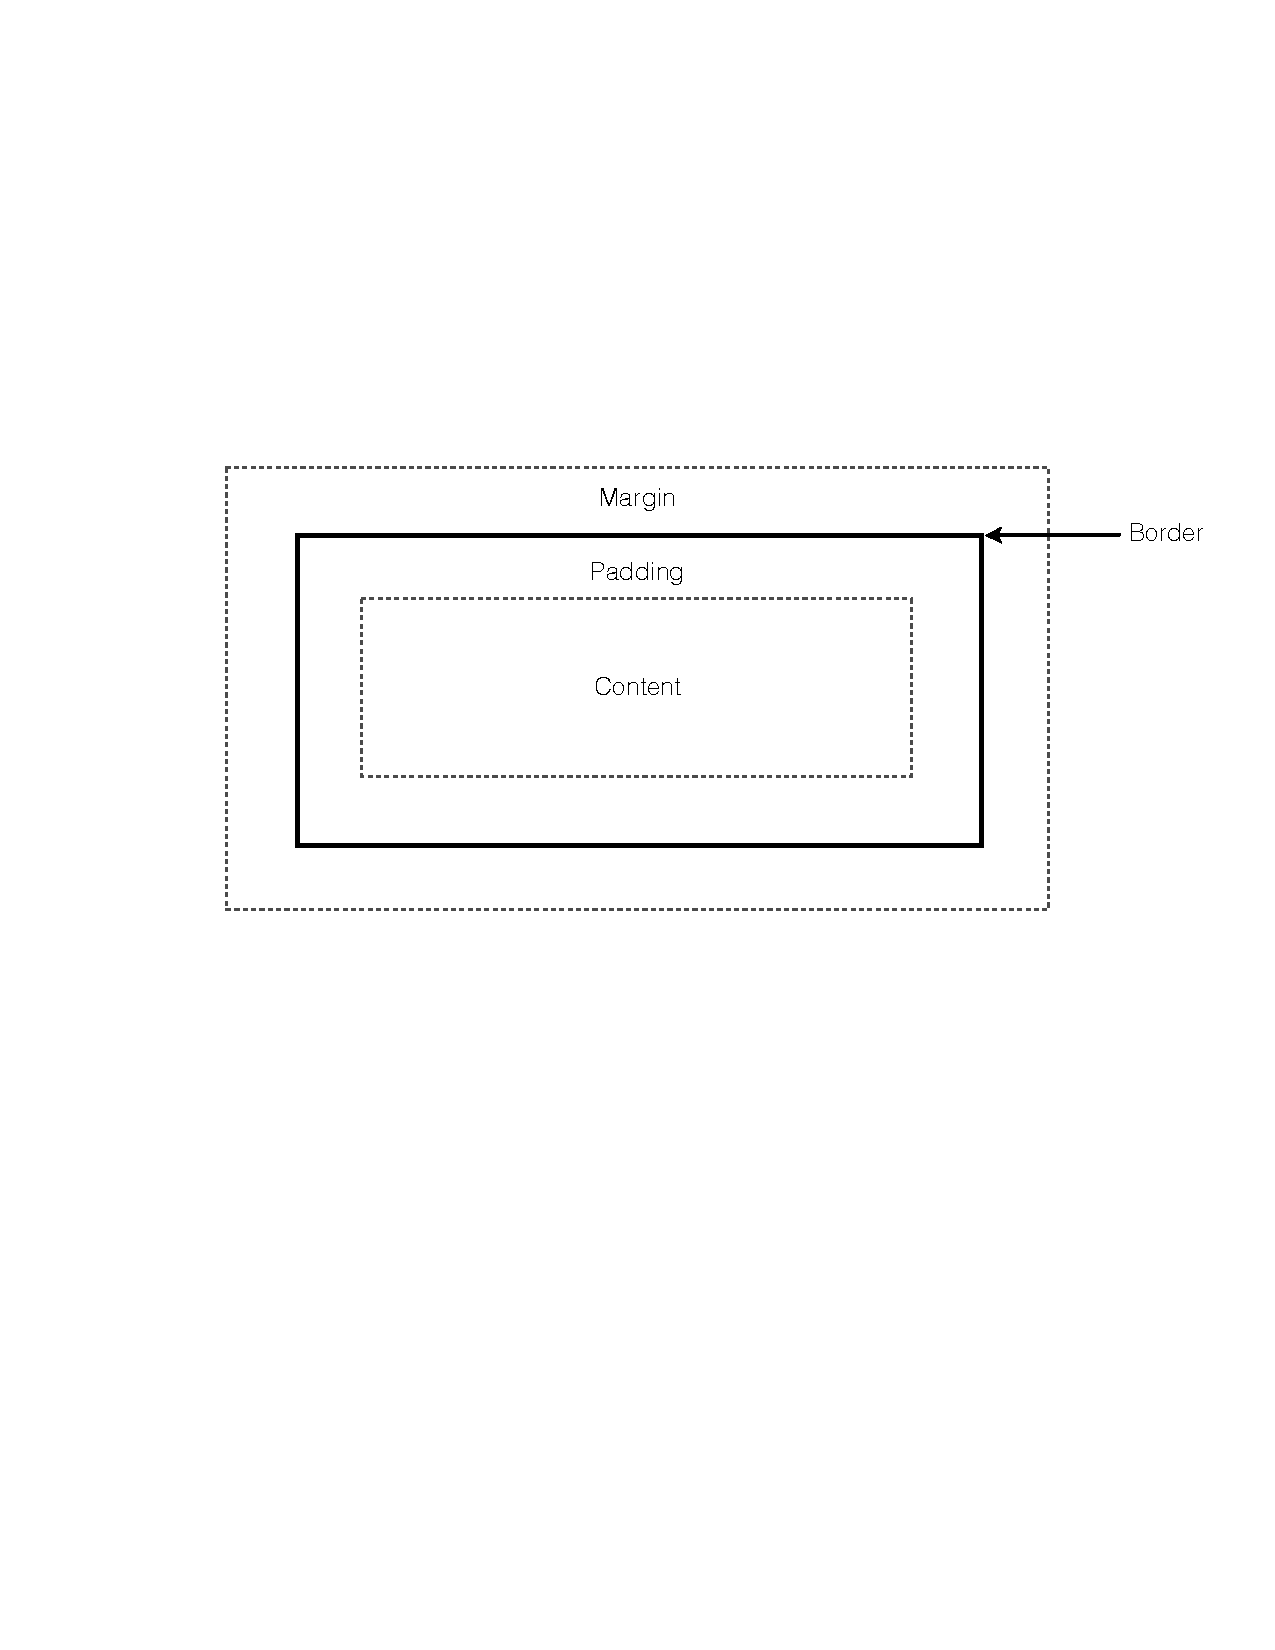
\includegraphics[width=\textwidth]{box_model}
	\caption{The Box Model}
	\label{fig:box_model}
\end{figure}

One should use \emph{margin} when there should be spacing between elements. How ever if one would like spacing from the content of the element to border of the element, \emph{padding} should be used.

